% Task 5: raise the price. Ciphertext from Task5/tamper.py; the invoice format from the README.
% CHECKED (python3, Task5/server.py): the ciphertext D2 3F BF D0 9C 33 F1 9D decrypts to "00000010";
%   XOR on the first byte only changes the first digit. The value of x is the result of the task: not shown.
\documentclass[12pt,tikz,border=6pt]{standalone}
% Shared preamble of the task figures of Lecture 1.
% The colours and styles are copied from the preamble of ../main.tex (keep them in sync).
\usepackage{lmodern}
\usepackage[T1]{fontenc}
\renewcommand{\familydefault}{\sfdefault}
\usepackage{amsmath,amssymb}
\usepackage{xcolor}
\usepackage{fontawesome5}
\usetikzlibrary{arrows.meta, calc, positioning, fit, decorations.pathreplacing, decorations.pathmorphing, backgrounds}

% ---------- template ----------
\definecolor{DeepBlue}{HTML}{283593}
\definecolor{AccentOrange}{HTML}{EB5A14}
\definecolor{LightGray}{HTML}{F5F6FA}
% ---------- actors and categories (S1 to S6) ----------
\definecolor{sIndigo}{HTML}{5C6BC0}   % the sender
\definecolor{sPink}{HTML}{EC407A}     % the attacker
\definecolor{sViolet}{HTML}{7E57C2}   % plaintext
\definecolor{sAmber}{HTML}{FFB300}    % key and keystream
\definecolor{sTeal}{HTML}{26A69A}     % the receiver
\definecolor{sBrown}{HTML}{8D6E63}    % ciphertext
\definecolor{sPinkText}{HTML}{C2185B}
\definecolor{sAmberText}{HTML}{A06A00}
\definecolor{sTealText}{HTML}{00796B}
% ---------- actions and results ----------
\definecolor{aExec}{HTML}{43A047}
\definecolor{aRead}{HTML}{1E88E5}
\definecolor{aWrite}{HTML}{E53935}
% ---------- neutral ----------
\definecolor{nInk}{HTML}{37474F}
\definecolor{nLine}{HTML}{90A4AE}
\definecolor{nLight}{HTML}{CFD8DC}
\definecolor{nFill}{HTML}{ECEFF1}
\definecolor{nIdle}{HTML}{E0E0E0}

% ---------- TikZ styles (as in main.tex; byte cells a little larger for the web) ----------
\tikzset{
  hw/.style={draw=nLine, thick, fill=nFill, text=nInk, rounded corners=3pt, align=center, inner sep=4pt},
  hwmain/.style={draw=nInk, thick, fill=nInk, text=white, rounded corners=3pt, align=center, inner sep=4pt},
  cell/.style={draw=nLine, thick, fill=white, text=nInk, font=\ttfamily\small},
  cellfree/.style={cell, dashed, draw=nLight},
  container/.style={draw=nLine, thick, dashed, rounded corners=5pt},
  actor/.style={fill=#1, draw=#1, text=white, rounded corners=3pt, align=center, font=\small\bfseries, inner sep=5pt},
  actorlight/.style={fill=#1!15, draw=#1, thick, text=nInk, rounded corners=3pt, align=center, inner sep=5pt},
  data/.style={-{Stealth}, very thick, nInk},
  flow/.style={-{Stealth}, very thick, DeepBlue},
  annot/.style={draw=AccentOrange, line width=1.6pt, rounded corners=3pt},
  byte/.style={draw=nLine, thick, fill=white, text=nInk, font=\ttfamily\small,
    minimum width=0.8cm, minimum height=0.62cm, inner sep=1pt, rounded corners=1.5pt},
  ptb/.style={byte, fill=sViolet!15, draw=sViolet},
  ksb/.style={byte, fill=sAmber!25, draw=sAmber},
  ctb/.style={byte, fill=sBrown!15, draw=sBrown},
  unk/.style={byte, fill=white, dashed, text=sViolet},
  rowlabel/.style={font=\small\bfseries, text=nInk, anchor=east},
  note/.style={font=\small, text=nInk},
  bigxor/.style={circle, draw=nInk, very thick, fill=white, inner sep=0pt, minimum size=0.8cm, font=\Large},
  radio/.style={-{Stealth}, very thick, nInk, decorate,
    decoration={snake, amplitude=1.2pt, segment length=7pt, post length=4pt}},
  % a white card behind the whole figure, so that it stays readable in a dark theme
  card/.style={show background rectangle, background rectangle/.style={fill=white, draw=none}, inner frame sep=8pt},
}
% a row of bytes: \byterow{x of the first cell}{y}{style}{list of values}{step between cells}
\newcommand{\byterow}[5]{%
  \expandafter\def\expandafter\brlist\expandafter{#4}%
  \foreach \v [count=\k from 0] in \brlist {
    \node[#3] at ({#1+#5*\k},#2) {\v};
  }}
% the generator / cipher box: dark, with cogs. \cogbox{name}{position}{label}{width}
\newcommand{\cogbox}[4]{%
  \node[hwmain, minimum width=#4, minimum height=1.3cm] (#1) at (#2) {};
  \node[text=white, font=\Large] at ([yshift=0.22cm]#1.center) {\faCogs};
  \node[text=white, font=\small\bfseries] at ([yshift=-0.32cm]#1.center) {#3};}
\newcommand{\ok}{\textcolor{aExec}{\faCheck}}
\newcommand{\nok}{\textcolor{aWrite}{\faTimes}}
\newcommand{\badge}[1]{\tikz[baseline=(b.base)]\node[circle,fill=AccentOrange,text=white,
  inner sep=1.5pt,font=\bfseries\footnotesize] (b) {#1};}

% an invoice on paper: \invoice{name}{position}{amount}
\newcommand{\invoice}[3]{%
  \node[draw=nLine, thick, fill=white, minimum width=2.5cm, minimum height=2.9cm, rounded corners=1pt] (#1) at (#2) {};
  \node[font=\small\bfseries, text=nInk, anchor=north] at ([yshift=-0.12cm]#1.north) {INVOICE};
  \foreach \d in {0.75,0.98,1.21} \draw[nLight, thick] ([shift={(0.25,-\d)}]#1.north west) -- ([shift={(-0.25,-\d)}]#1.north east);
  \node[font=\scriptsize, text=nInk, anchor=south west] at ([shift={(0.15,0.6)}]#1.south west) {to pay (PLN):};
  \node[font=\ttfamily\normalsize\bfseries, text=nInk, anchor=south] at ([yshift=0.15cm]#1.south) {#3};}
\begin{document}
\pagecolor{white}
\begin{tikzpicture}[>=Stealth]
  \def\dx{1.0}
  \def\xs{5.2}
  % the way of the message
  \node[actor=sIndigo, minimum width=2.4cm, minimum height=0.9cm] (a) at (1.0,3.0) {\faUser\ Alice};
  \node[actor=sTeal, minimum width=2.4cm, minimum height=0.9cm] (b) at (17.2,3.0) {\faUser\ Bob};
  \draw[data] (a) -- node[above, note] {ciphertext} (7.9,3.0);
  \draw[data] (10.5,3.0) -- node[above, note] {changed ciphertext} (b);
  \node[circle, fill=sPink, text=white, minimum size=1.1cm, font=\Large] (x) at (9.2,3.0) {\faUserSecret};
  \node[font=\small\bfseries, text=sPinkText] at (9.2,2.15) {you are Mallory: no key, but you can change bytes};

  % what Alice wrote
  \invoice{i1}{1.0,-0.4}{00000010}
  \node[note] at (1.0,-2.15) {Alice: 10 PLN};
  % the bytes
  \node[rowlabel, font=\small, text=gray] at ({\xs-0.55},1.15) {byte};
  \foreach \k in {0,...,7} \node[font=\small, text=gray] at ({\xs+\dx*\k},1.15) {\k};
  \node[rowlabel] at ({\xs-0.55},0.6) {plaintext};
  \byterow{\xs}{0.6}{ptb}{30,30,30,30,30,30,31,30}{\dx}
  \node[font=\small, text=sViolet, anchor=west] at ({\xs+7.55*\dx},0.6) {= \texttt{"00000010"}};
  \node[rowlabel] at ({\xs-0.55},-0.3) {ciphertext};
  \byterow{\xs}{-0.3}{ctb}{D2,3F,BF,D0,9C,33,F1,9D}{\dx}
  \node[rowlabel] at ({\xs-0.55},-1.2) {XOR};
  \node[byte, draw=AccentOrange, line width=1.4pt, text=AccentOrange, font=\ttfamily\normalsize\bfseries] at (\xs,-1.2) {x};
  \foreach \k in {1,...,7} \node[cellfree, minimum width=0.8cm, minimum height=0.62cm, font=\ttfamily\small, text=nLine] at ({\xs+\dx*\k},-1.2) {00};
  \draw[nInk, thick] ({\xs-0.45},-1.65) -- ({\xs+7.45*\dx},-1.65);
  \node[rowlabel] at ({\xs-0.55},-2.15) {decrypted};
  \node[ptb, draw=AccentOrange, line width=1.4pt, font=\ttfamily\normalsize\bfseries] at (\xs,-2.15) {35};
  \byterow{\xs+\dx}{-2.15}{ptb}{30,30,30,30,30,31,30}{\dx}
  \node[font=\small, text=sViolet, anchor=west] at ({\xs+7.55*\dx},-2.15) {= \texttt{"50000010"}};
  \draw[annot] ({\xs-0.5},-2.55) rectangle ({\xs+0.5},0.95);

  % what Bob accepts
  \invoice{i2}{17.2,-0.4}{50000010}
  \node[font=\small\bfseries, text=sTealText] at (17.2,-2.15) {Bob accepts it \ok};
  \node[note, anchor=north, align=center] at (9.2,-2.75)
    {A change in the ciphertext lands on \textbf{the same byte} of the plaintext: \ \texttt{(C XOR x)} decrypts to \texttt{P XOR x}.\\ Which \texttt{x} turns \texttt{0x30} (the digit 0) into \texttt{0x35} (the digit 5)?};
\end{tikzpicture}
\end{document}
